%%%%%%%%%%%%%%%%%%%%%%%%%%%%%%%%%%
% !TEX program = xelatex
% !Mode:: "TeX:UTF-8"
%%%%%%%%%%%%%%%%%%%%%%%%%%%%%%%%%%
\documentclass{mactexbook}
\newif\ifattachpdffile
\newif\ifLinuxProcess
\newif\ifLinuxMemory
\newif\ifLinuxIO
\newif\ifLinuxLock
\attachpdffilefalse  %false 控制编译时不添加 视频附件
%\attachpdffiletrue  %true 添加 视频附件
%\LinuxProcesstrue
\LinuxLocktrue


\wdtexbooktheme{bodie} %
\wdtexbookcolor{green} % green, violet, print
\ifattachpdffile
\wdtitle{wangfan的Linux进程笔记--完整版}
%\wdedition{\href{https://github.com/wangfanstar/LinuxProcessNote}{\LaTeX}\quad \href{https://www.wangfanstar.top/categories/宋宝华/}{Web}\quad}
\wdedition{20180522}
\else
\wdtitle{wangfan的Linux进程笔记--精简版}
\wdedition{20180522}
\fi
\wdfirstauthor{linux 进程管理 -- 宋宝华}
\wdfirstinstitute{}
\wdsecondauthor{wangfanstar@163.com}
\wdsecondinstitute{}
%\wdsecondinstitute{\today}
\wdthirdauthor{\today}
\wdthirdinstitute{}

%%%%%%%%%%%%%%%%%%%%%%%%%%%%%%%%
%%%%%%%%%%%%%%%%%%%%%%%%%%%%%%%%%%
% !TEX program = xelatex
% !Mode:: "TeX:UTF-8"
%%%%%%%%%%%%%%%%%%%%%%%%%%%%%%%%%%
%% 去除英文的figure 和 table 标记
\renewcommand\figurename{}
\renewcommand\tablename{}
\renewcommand\theexample{ \arabic{chapter}-\arabic{example}~}%将例号1.1改成1-1
\renewcommand\examplename{应用}
%% 去掉章节标题中的数字
\renewcommand{\chaptermark}[1]{\markboth{\chaptername \ #1}{}}

\newcommand\song[1]{{\songti{#1}}}
\newcommand\fs[1]{{\fangsong{#1}}}
\newcommand\hei[1]{{\heiti\textbf{#1}}}
\newcommand\kai[1]{{\kaishu\emph{#1}}}
\newcommand\li[1]{{\lishu{#1}}}
\newcommand\you[1]{{\youyuan{#1}}}


\DefineVerbatimEnvironment{latexcmd}{Verbatim}
{gobble=0,rulecolor=\color{black},formatcom=\color{blue},samepage=true,numbers=none,numbersep=0mm,
frame=single,framerule=0.1pt,label=bash \quad 命令,fontsize=\small}

\definecolor{lightgray}{rgb}{0.75,0.75, 0.75}
\definecolor{grass}{rgb}{0.00,0.50,0.25}   %用于程序语言
\definecolor{lightgreen}{rgb}{0.93,1.00,0.93}

\definecolor{lightred}{rgb}{1.00,0.50,0.50}
\definecolor{deepyellow}{rgb}{0.91,0.91,0.00}
\definecolor{lightyellow}{rgb}{1,1,0.9}%浅黄,适合作代码框背景
\definecolor{deepgreen}{rgb}{0.00,0.50,0.00} %深绿,适合作代码注释
\definecolor{deepblue}{rgb}{0.00,0.40,0.40}
\definecolor{lightblue}{rgb}{0.50,0.50,1.00} %浅蓝
\definecolor{whiteblue}{rgb}{0.82,0.82,1.00} %蓝白


\definecolor{shadecolor}{rgb}{0.92,0.92,0.92} %文本背景色
%\definecolor{backcolor}{rgb}{1,1,0.95} %米黄色背景
\definecolor{backcolor}{rgb}{1,1,0.955} %黄色背景

\definecolor{bg-color}{rgb}{0.96,1,0.95}
\definecolor{shadecolor}{rgb}{0.96,1,0.95} %文本背景色
\definecolor{info}{rgb}{1.00,0.50,0.50} %粉色
\definecolor{txt-color}{HTML}{000000}
\definecolor{builtin}{HTML}{DA70D6}
\definecolor{comment}{HTML}{B22222}
\definecolor{comment-delimiter}{HTML}{B22222}
\definecolor{constant}{HTML}{5F9EA0}
\definecolor{function-name}{HTML}{0000FF}
\definecolor{keyword}{HTML}{a020F0}
\definecolor{string}{HTML}{BC8F8F}
\definecolor{type}{HTML}{228B22}
\definecolor{variable-name}{HTML}{B8860B}
\definecolor{brick}{HTML}{7B0C00}
\definecolor{shadecolor}{rgb}{0.92,0.92,0.92}

\usepackage[listings]{tcolorbox}
\usepackage{framed}

\usepackage{dirtree}
\usepackage{listings}
% 语言定义
\lstdefinelanguage{Asymptote}{alsoletter={},
sensitive=true,% 大小写
keywords={and,controls,tension,atleast,curl,if,else,while,for,do,return,break,continue,struct,typedef,new,access,import,unravel,from,include,quote,static,public,private,restricted,this,explicit,true,false,null,cycle,newframe,operator},
keywords=[2]{Braid,FitResult,Label,Legend,Segment,Solution,TreeNode,abscissa,arc,arrowhead,binarytree,binarytreeNode,block,bool,bool3,bounds,bqe,circle,conic,coord,coordsys,cputime,ellipse,file,filltype,frame,grid3,guide,horner,hsv,hyperbola,indexedTransform,int,inversion,key,light,line,linefit,marginT,marker,mass,object,pair,parabola,path,path3,pen,picture,point,position,projection,real,revolution,scaleT,scientific,segment,side,slice,solution,splitface,string,surface,tensionSpecifier,ticklocate,ticksgridT,tickvalues,transform,transformation,tree,triangle,trilinear,triple,vector,vertex,void},
keywords=[3]{AND,Arc,ArcArrow,ArcArrows,Arrow,Arrows,Automatic,AvantGarde,BBox,BWRainbow,BWRainbow2,Bar,Bars,BeginArcArrow,BeginArrow,BeginBar,BeginDotMargin,BeginMargin,BeginPenMargin,Blank,Bookman,Bottom,BottomTop,Bounds,Break,Broken,BrokenLog,CLZ,CTZ,Ceil,Circle,CircleBarIntervalMarker,Cos,Courier,CrossIntervalMarker,DefaultFormat,DefaultLogFormat,Degrees,Dir,DotMargin,DotMargins,Dotted,Draw,Drawline,Embed,EndArcArrow,EndArrow,EndBar,EndDotMargin,EndMargin,EndPenMargin,Fill,FillDraw,Floor,Format,Full,Gaussian,Gaussrand,Gaussrandpair,Gradient,Grayscale,Helvetica,Hermite,HookHead,InOutTicks,InTicks,Jn,Label,Landscape,Left,LeftRight,LeftTicks,Legend,Linear,Link,Log,LogFormat,Margin,Margins,Mark,MidArcArrow,MidArrow,NOT,NewCenturySchoolBook,NoBox,NoMargin,NoModifier,NoTicks,NoTicks3,NoZero,NoZeroFormat,None,OR,OmitFormat,OmitTick,OmitTickInterval,OmitTickIntervals,OutTicks,Ox,Oy,Palatino,PaletteTicks,Pen,PenMargin,PenMargins,Pentype,Portrait,RadialShade,RadialShadeDraw,Rainbow,Range,Relative,Right,RightTicks,Rotate,Round,SQR,Scale,ScaleX,ScaleY,ScaleZ,Seascape,Segment,Shift,Sin,Slant,Spline,StickIntervalMarker,Straight,Symbol,Tan,TeXify,Ticks,Ticks3,TildeIntervalMarker,TimesRoman,Top,TrueMargin,UnFill,UpsideDown,Wheel,X,XEquals,XOR,XY,XYEquals,XYZero,XYgrid,XZEquals,XZZero,XZero,XZgrid,Y,YEquals,YXgrid,YZ,YZEquals,YZZero,YZero,YZgrid,Yn,Z,ZX,ZXgrid,ZYgrid,ZapfChancery,ZapfDingbats,_begingroup3,_cputime,_draw,_eval,_image,_labelpath,_projection,_strokepath,_texpath,aCos,aSin,aTan,abort,abs,accel,acos,acosh,acot,acsc,activatequote,add,addArrow,addMargins,addSaveFunction,addnode,addnodes,addpenarc,addpenline,adjust,alias,align,all,altitude,angabscissa,angle,angpoint,animate,annotate,anticomplementary,antipedal,apply,approximate,arc,arcarrowsize,arccircle,arcdir,arcfromcenter,arcfromfocus,arclength,arcnodesnumber,arcpoint,arcsubtended,arcsubtendedcenter,arctime,arctopath,array,arrow,arrow2,arrowbase,arrowbasepoints,arrowsize,asec,asin,asinh,ask,assert,asy,asycode,asydir,asyfigure,asyfilecode,asyinclude,asywrite,atan,atan2,atanh,atbreakpoint,atexit,atime,attach,attract,atupdate,autoformat,autoscale,autoscale3,axes,axes3,axialshade,axis,axiscoverage,azimuth,babel,background,bangles,bar,barmarksize,barsize,basealign,baseline,bbox,beep,begin,beginclip,begingroup,beginpoint,between,bevel,bezier,bezierP,bezierPP,bezierPPP,bezulate,bibliography,bibliographystyle,binarytree,binarytreeNode,binomial,binput,bins,bisector,bisectorpoint,bispline,blend,blockconnector,boutput,box,bqe,breakpoint,breakpoints,brick,buildRestoreDefaults,buildRestoreThunk,buildcycle,bulletcolor,byte,canonical,canonicalcartesiansystem,cartesiansystem,case1,case2,case3,case4,cbrt,cd,ceil,center,centerToFocus,centroid,cevian,change2,changecoordsys,checkSegment,checkconditionlength,checker,checkincreasing,checklengths,checkposition,checktriangle,choose,circle,circlebarframe,circlemarkradius,circlenodesnumber,circumcenter,circumcircle,clamped,clear,clip,clipdraw,close,cmyk,code,colatitude,collect,collinear,color,colorless,colors,colorspace,comma,compassmark,complement,complementary,concat,concurrent,cone,conic,conicnodesnumber,conictype,conj,connect,connected,connectedindex,containmentTree,contains,contour,contour3,contouredges,controlSpecifier,convert,coordinates,coordsys,copy,cos,cosh,cot,countIntersections,cputime,crop,cropcode,cross,crossframe,crosshatch,crossmarksize,csc,cubicroots,curabscissa,curlSpecifier,curpoint,currentarrow,currentexitfunction,currentmomarrow,currentpolarconicroutine,curve,cut,cutafter,cutbefore,cyclic,cylinder,deactivatequote,debugger,deconstruct,defaultdir,defaultformat,defaultpen,defined,degenerate,degrees,delete,deletepreamble,determinant,diagonal,diamond,diffdiv,dir,dirSpecifier,dirtime,display,distance,divisors,do_overpaint,dot,dotframe,dotsize,downcase,draw,drawAll,drawDoubleLine,drawFermion,drawGhost,drawGluon,drawMomArrow,drawPRCcylinder,drawPRCdisk,drawPRCsphere,drawPRCtube,drawPhoton,drawScalar,drawVertex,drawVertexBox,drawVertexBoxO,drawVertexBoxX,drawVertexO,drawVertexOX,drawVertexTriangle,drawVertexTriangleO,drawVertexX,drawarrow,drawarrow2,drawline,drawtick,duplicate,elle,ellipse,ellipsenodesnumber,embed,embed3,empty,enclose,end,endScript,endclip,endgroup,endgroup3,endl,endpoint,endpoints,eof,eol,equation,equations,erase,erasestep,erf,erfc,error,errorbar,errorbars,eval,excenter,excircle,exit,exitXasyMode,exitfunction,exp,expfactors,expi,expm1,exradius,extend,extension,extouch,fabs,factorial,fermat,fft,fhorner,figure,file,filecode,fill,filldraw,filloutside,fillrule,filltype,find,finite,finiteDifferenceJacobian,firstcut,firstframe,fit,fit2,fixedscaling,floor,flush,fmdefaults,fmod,focusToCenter,font,fontcommand,fontsize,foot,format,frac,frequency,fromCenter,fromFocus,fspline,functionshade,gamma,generate_random_backtrace,generateticks,gergonne,getc,getint,getpair,getreal,getstring,gettriple,gluon,gouraudshade,graph,graphic,gray,grestore,grid,grid3,gsave,halfbox,hatch,hdiffdiv,hermite,hex,histogram,history,hline,hprojection,hsv,hyperbola,hyperbolanodesnumber,hyperlink,hypot,identity,image,incenter,incentral,incircle,increasing,incrementposition,indexedTransform,indexedfigure,initXasyMode,initdefaults,input,inradius,insert,inside,integrate,interactive,interior,interp,interpolate,intersect,intersection,intersectionpoint,intersectionpoints,intersections,intouch,inverse,inversion,invisible,is3D,isCCW,isDuplicate,isogonal,isogonalconjugate,isotomic,isotomicconjugate,isparabola,italic,item,key,kurtosis,kurtosisexcess,label,labelaxis,labelmargin,labelpath,labels,labeltick,labelx,labelx3,labely,labely3,labelz,labelz3,lastcut,latex,latitude,latticeshade,layer,layout,ldexp,leastsquares,legend,legenditem,length,lexorder,lift,light,limits,line,linear,linecap,lineinversion,linejoin,linemargin,lineskip,linetype,linewidth,link,list,lm_enorm,lm_evaluate_default,lm_lmdif,lm_lmpar,lm_minimize,lm_print_default,lm_print_quiet,lm_qrfac,lm_qrsolv,locale,locate,locatefile,location,log,log10,log1p,logaxiscoverage,longitude,lookup,magnetize,makeNode,makedraw,makepen,map,margin,markangle,markangleradius,markanglespace,markarc,marker,markinterval,marknodes,markrightangle,markuniform,mass,masscenter,massformat,math,max,max3,maxbezier,maxbound,maxcoords,maxlength,maxratio,maxtimes,mean,medial,median,midpoint,min,min3,minbezier,minbound,minipage,minratio,mintimes,miterlimit,momArrowPath,momarrowsize,monotonic,multifigure,nativeformat,natural,needshipout,newl,newpage,newslide,newton,newtree,nextframe,nextnormal,nextpage,nib,nodabscissa,none,norm,normalvideo,notaknot,nowarn,numberpage,nurb,object,offset,onpath,opacity,opposite,orientation,orig_circlenodesnumber,orig_circlenodesnumber1,orig_draw,orig_ellipsenodesnumber,orig_ellipsenodesnumber1,orig_hyperbolanodesnumber,orig_parabolanodesnumber,origin,orthic,orthocentercenter,outformat,outline,outname,outprefix,output,overloadedMessage,overwrite,pack,pad,pairs,palette,parabola,parabolanodesnumber,parallel,parallelogram,partialsum,path,path3,pattern,pause,pdf,pedal,periodic,perp,perpendicular,perpendicularmark,phantom,phi1,phi2,phi3,photon,piecewisestraight,point,polar,polarconicroutine,polargraph,polygon,postcontrol,postscript,pow10,ppoint,prc,prc0,precision,precontrol,prepend,print_random_addresses,project,projection,purge,pwhermite,quadrant,quadraticroots,quantize,quarticroots,quotient,radialshade,radians,radicalcenter,radicalline,radius,rand,randompath,rd,readline,realmult,realquarticroots,rectangle,rectangular,rectify,reflect,relabscissa,relative,relativedistance,reldir,relpoint,reltime,remainder,remark,removeDuplicates,rename,replace,report,resetdefaultpen,restore,restoredefaults,reverse,reversevideo,rf,rfind,rgb,rgba,rgbint,rms,rotate,rotateO,rotation,round,roundbox,roundedpath,roundrectangle,same,samecoordsys,sameside,sample,save,savedefaults,saveline,scale,scale3,scaleO,scaleT,scaleless,scientific,search,searchindex,searchtree,sec,secondaryX,secondaryY,seconds,section,sector,seek,seekeof,segment,sequence,setcontour,setpens,sgn,sgnd,sharpangle,sharpdegrees,shift,shiftless,shipout,shipout3,show,side,simeq,simpson,sin,single,sinh,size,size3,skewness,skip,slant,sleep,slope,slopefield,solve,solveBVP,sort,sourceline,sphere,split,sqrt,square,srand,standardizecoordsys,startScript,startTrembling,stdev,step,stickframe,stickmarksize,stickmarkspace,stop,straight,straightness,string,stripdirectory,stripextension,stripfile,stripsuffix,strokepath,subdivide,subitem,subpath,substr,sum,surface,symmedial,symmedian,system,tab,tableau,tan,tangent,tangential,tangents,tanh,tell,tensionSpecifier,tensorshade,tex,texcolor,texify,texpath,texpreamble,texreset,texshipout,texsize,textpath,thick,thin,tick,tickMax,tickMax3,tickMin,tickMin3,ticklabelshift,ticklocate,tildeframe,tildemarksize,tile,tiling,time,times,title,titlepage,topbox,transform,transformation,transpose,tremble,trembleFuzz,tremble_circlenodesnumber,tremble_circlenodesnumber1,tremble_draw,tremble_ellipsenodesnumber,tremble_ellipsenodesnumber1,tremble_hyperbolanodesnumber,tremble_marknodes,tremble_markuniform,tremble_parabolanodesnumber,triangle,triangleAbc,triangleabc,triangulate,tricoef,tridiagonal,trilinear,trim,trueMagnetize,truepoint,tube,uncycle,unfill,uniform,unique,unit,unitrand,unitsize,unityroot,unstraighten,upcase,updatefunction,uperiodic,upscale,uptodate,usepackage,usersetting,usetypescript,usleep,value,variance,variancebiased,vbox,vector,vectorfield,verbatim,view,vline,vperiodic,vprojection,warn,warning,windingnumber,write,xaxis,xaxis3,xaxis3At,xaxisAt,xequals,xinput,xlimits,xoutput,xpart,xscale,xscaleO,xtick,xtick3,xtrans,yaxis,yaxis3,yaxis3At,yaxisAt,yequals,ylimits,ypart,yscale,yscaleO,ytick,ytick3,ytrans,zaxis3,zaxis3At,zero,zero3,zlimits,zpart,ztick,ztick3,ztrans},
keywords=[4]{AliceBlue,Align,Allow,AntiqueWhite,Apricot,Aqua,Aquamarine,Aspect,Azure,BeginPoint,Beige,Bisque,Bittersweet,Black,BlanchedAlmond,Blue,BlueGreen,BlueViolet,Both,Break,BrickRed,Brown,BurlyWood,BurntOrange,CCW,CW,CadetBlue,CarnationPink,Center,Centered,Cerulean,Chartreuse,Chocolate,Coeff,Coral,CornflowerBlue,Cornsilk,Crimson,Crop,Cyan,Dandelion,DarkBlue,DarkCyan,DarkGoldenrod,DarkGray,DarkGreen,DarkKhaki,DarkMagenta,DarkOliveGreen,DarkOrange,DarkOrchid,DarkRed,DarkSalmon,DarkSeaGreen,DarkSlateBlue,DarkSlateGray,DarkTurquoise,DarkViolet,DeepPink,DeepSkyBlue,DefaultHead,DimGray,DodgerBlue,Dotted,Down,Draw,E,ENE,EPS,ESE,E_Euler,E_PC,E_RK2,E_RK3BS,Emerald,EndPoint,Euler,Fill,FillDraw,FireBrick,FloralWhite,ForestGreen,Fuchsia,Gainsboro,GhostWhite,Gold,Goldenrod,Gray,Green,GreenYellow,Honeydew,HookHead,Horizontal,HotPink,I,IgnoreAspect,IndianRed,Indigo,Ivory,JOIN_IN,JOIN_OUT,JungleGreen,Khaki,LM_DWARF,LM_MACHEP,LM_SQRT_DWARF,LM_SQRT_GIANT,LM_USERTOL,Label,Lavender,LavenderBlush,LawnGreen,Left,LeftJustified,LeftSide,LemonChiffon,LightBlue,LightCoral,LightCyan,LightGoldenrodYellow,LightGreen,LightGrey,LightPink,LightSalmon,LightSeaGreen,LightSkyBlue,LightSlateGray,LightSteelBlue,LightYellow,Lime,LimeGreen,Linear,Linen,Log,Logarithmic,Magenta,Mahogany,Mark,MarkFill,Maroon,Max,MediumAquamarine,MediumBlue,MediumOrchid,MediumPurple,MediumSeaGreen,MediumSlateBlue,MediumSpringGreen,MediumTurquoise,MediumVioletRed,Melon,MidPoint,MidnightBlue,Min,MintCream,MistyRose,Moccasin,Move,MoveQuiet,Mulberry,N,NE,NNE,NNW,NW,NavajoWhite,Navy,NavyBlue,NoAlign,NoCrop,NoFill,NoSide,OldLace,Olive,OliveDrab,OliveGreen,Orange,OrangeRed,Orchid,Ox,Oy,PC,PaleGoldenrod,PaleGreen,PaleTurquoise,PaleVioletRed,PapayaWhip,Peach,PeachPuff,Periwinkle,Peru,PineGreen,Pink,Plum,PowderBlue,ProcessBlue,Purple,RK2,RK3,RK3BS,RK4,RK5,RK5DP,RK5F,RawSienna,Red,RedOrange,RedViolet,Rhodamine,Right,RightJustified,RightSide,RosyBrown,RoyalBlue,RoyalPurple,RubineRed,S,SE,SSE,SSW,SW,SaddleBrown,Salmon,SandyBrown,SeaGreen,Seashell,Sepia,Sienna,Silver,SimpleHead,SkyBlue,SlateBlue,SlateGray,Snow,SpringGreen,SteelBlue,Suppress,SuppressQuiet,Tan,TeXHead,Teal,TealBlue,Thistle,Ticksize,Tomato,Turquoise,UnFill,Up,VERSION,Value,Vertical,Violet,VioletRed,W,WNW,WSW,Wheat,White,WhiteSmoke,WildStrawberry,XYAlign,YAlign,Yellow,YellowGreen,YellowOrange,addpenarc,addpenline,align,allowstepping,angularsystem,animationdelay,appendsuffix,arcarrowangle,arcarrowfactor,arrow2sizelimit,arrowangle,arrowbarb,arrowdir,arrowfactor,arrowhookfactor,arrowlength,arrowsizelimit,arrowtexfactor,authorpen,axis,axiscoverage,axislabelfactor,background,backgroundcolor,backgroundpen,barfactor,barmarksizefactor,basealign,baselinetemplate,beveljoin,bigvertexpen,bigvertexsize,black,blue,bm,bottom,bp,brown,bullet,byfoci,byvertices,camerafactor,chartreuse,circlemarkradiusfactor,circlenodesnumberfactor,circleprecision,circlescale,cm,codefile,codepen,codeskip,colorPen,coloredNodes,coloredSegments,conditionlength,conicnodesfactor,count,cputimeformat,crossmarksizefactor,currentcoordsys,currentlight,currentpatterns,currentpen,currentpicture,currentposition,currentprojection,curvilinearsystem,cuttings,cyan,darkblue,darkbrown,darkcyan,darkgray,darkgreen,darkgrey,darkmagenta,darkolive,darkred,dashdotted,dashed,datepen,dateskip,debuggerlines,debugging,deepblue,deepcyan,deepgray,deepgreen,deepgrey,deepmagenta,deepred,default,defaultControl,defaultS,defaultbackpen,defaultcoordsys,defaultexcursion,defaultfilename,defaultformat,defaultmassformat,defaultpen,diagnostics,differentlengths,dot,dotfactor,dotframe,dotted,doublelinepen,doublelinespacing,down,duplicateFuzz,edge,ellipsenodesnumberfactor,eps,epsgeo,epsilon,evenodd,extendcap,exterior,fermionpen,figureborder,figuremattpen,firstnode,firststep,foregroundcolor,fuchsia,fuzz,gapfactor,ghostpen,gluonamplitude,gluonpen,gluonratio,gray,green,grey,hatchepsilon,havepagenumber,heavyblue,heavycyan,heavygray,heavygreen,heavygrey,heavymagenta,heavyred,hline,hwratio,hyperbola,hyperbolanodesnumberfactor,identity4,ignore,inXasyMode,inch,inches,includegraphicscommand,inf,infinity,institutionpen,intMax,intMin,interior,invert,invisible,itempen,itemskip,itemstep,labelmargin,landscape,lastnode,left,legendhskip,legendlinelength,legendmargin,legendmarkersize,legendmaxrelativewidth,legendvskip,lightblue,lightcyan,lightgray,lightgreen,lightgrey,lightmagenta,lightolive,lightred,lightyellow,line,linemargin,lm_infmsg,lm_shortmsg,longdashdotted,longdashed,magenta,magneticPoints,magneticRadius,mantissaBits,markangleradius,markangleradiusfactor,markanglespace,markanglespacefactor,mediumblue,mediumcyan,mediumgray,mediumgreen,mediumgrey,mediummagenta,mediumred,mediumyellow,middle,minDistDefault,minblockheight,minblockwidth,mincirclediameter,minipagemargin,minipagewidth,minvertexangle,miterjoin,mm,momarrowfactor,momarrowlength,momarrowmargin,momarrowoffset,momarrowpen,monoPen,morepoints,nCircle,newbulletcolor,ngraph,nil,nmesh,nobasealign,nodeMarginDefault,nodesystem,nomarker,nopoint,noprimary,nullpath,nullpen,numarray,ocgindex,oldbulletcolor,olive,orange,origin,overpaint,page,pageheight,pagemargin,pagenumberalign,pagenumberpen,pagenumberposition,pagewidth,paleblue,palecyan,palegray,palegreen,palegrey,palemagenta,palered,paleyellow,parabolanodesnumberfactor,perpfactor,phi,photonamplitude,photonpen,photonratio,pi,pink,plain,plus,preamblenodes,pt,purple,r3,r4a,r4b,randMax,realDigits,realEpsilon,realMax,realMin,red,relativesystem,reverse,right,roundcap,roundjoin,royalblue,salmon,saveFunctions,scalarpen,sequencereal,settings,shipped,signedtrailingzero,solid,springgreen,sqrtEpsilon,squarecap,squarepen,startposition,stdin,stdout,stepfactor,stepfraction,steppagenumberpen,stepping,stickframe,stickmarksizefactor,stickmarkspacefactor,textpen,ticksize,tildeframe,tildemarksizefactor,tinv,titlealign,titlepagepen,titlepageposition,titlepen,titleskip,top,trailingzero,treeLevelStep,treeMinNodeWidth,treeNodeStep,trembleAngle,trembleFrequency,trembleRandom,tremblingMode,undefined,unitcircle,unitsquare,up,urlpen,urlskip,version,vertexpen,vertexsize,viewportmargin,viewportsize,vline,white,wye,xformStack,yellow,ylabelwidth,zerotickfuzz,zerowinding},
% otherkeywords={!,@,\$,\%,+,-,^,=,>,<,->,
% --,..,**,::,\@\@,\$\$,---,...},% 运算符等,但小心会与注释冲突
morecomment=[l]{//},% 注释
morecomment=[s]{/*}{*/},% 注释
morestring=[b]",% 字符串
morestring=[b]',% 字符串
}
% 定义别名
\lstalias{asy}{Asymptote}
\lstset{%extendedchars=false,% 解决中文跨页出错的问题;对 xetex 无用
language={Asymptote},
basewidth={.5em},
basicstyle={\ttfamily\footnotesize},%如果用 rmfamily 和 sffamily 在PDF中复制格式会多出很多空格
keywordstyle={\color{keyword}},
keywordstyle=[2]{\color{type}},
keywordstyle=[3]{\color{function-name}},
keywordstyle=[4]{\color{variable-name}},
commentstyle={\color{comment}},
stringstyle={\color{string}},
xleftmargin={0em},
xrightmargin={0em},
tabsize=8,
backgroundcolor={\color{shadecolor}},
% numbers=left,
numberstyle=\tiny,
showstringspaces=false, %不显示空格标记
stepnumber=1,
escapeinside=``,
numbersep=5pt}
%
\lstdefinestyle{lesscolor}{keywordstyle={\color{keyword!50!black}},
keywordstyle=[2]{\color{type!50!black}},
keywordstyle=[3]{\color{function-name!50!black}},
keywordstyle=[4]{\color{variable-name!50!black}},
commentstyle={\color{comment!50!black}},
stringstyle={\color{string!50!black}}}
%
%\def\oldvert{|} % 保存字符 | 的旧定义(其 catcode 在此定义读入时已确定)
%\lstMakeShortInline[style=lesscolor]\|
%
%
\def\inlinecode{\expandafter\lstinline[style=lesscolor]}

\endinput

%%% Local Variables:
%%% TeX-master: "main"
%%% End:


%%%%%%%%%%%%%%%%%%%%%%%%%%%%%%%%

\begin{document}
\wdmaketitle

\shorttoc{目录大纲}{0}

\tableofcontents

%====== be sure to add this part ====%
\switchgeometry
\wdstartdoc
% \addtocontents{toc}{\protect\begin{multicols}{2}}
% \setcounter{page}{1}
% \renewcommand{\thepage}{\arabic{page}}
% ====== be sure to add this part ====%

\newcommand{\videoattach}[3]
{\ifattachpdffile
\textattachfile{#1}{\textcolor[rgb]{0.00,0.00,0.55}{\textbf{#2}}}
\else
{\heiti{#2链接:}}\url{#3}
\fi
}
%\renewcommand{\textbf}[1]{\heiti{#1}}

\ifLinuxProcess


\partabstractfp{文档是我在学习宋宝华老师2018.05.22开始的4天进程课程中做的笔记,内容大部分来自老师的课程,
其中根据自己的理解调整了章节架构和顺序,有些内容会和实际上课的有差异。
}
\partabstractrp{\textbf{文档相关附件}:因视频文件占用空间太大,约140Mb,本文档分有视频附件完整版和无视频附件的精简版,有视频附件的完整版在支持PDF附件的阅读器中直接双击PDF文档即可观看视频,无视频附件版提供相关文件链接。}
\partabstractlettrine{本}{} % the first word of the abstract

\part{前言}

%%% Local Variables:
%%% TeX-master: "main"
%%% End:

\partabstractfp{进程有6种状态。\\~\\~\\考虑以下问题:\\1. 僵尸态是什么?\\2. 如何进入停止态?\\3. 什么是内存泄露?\\4. task\_struct与task\_struct之间的关系是什么?}
\partabstractrp{{\heiti{练习题:}}\\1. fork的例子 \\2. life-period例子,观察僵尸\\3.用cpulimit控制cpu利用率}
\partabstractlettrine{L}{inux} % the first word of the abstract

\part{进程课第1天}

\chapter{进程的代码结构}
\section{进程控制块PCB与task\_struct}
进程是一个资源封装的单位,资源指占用的内存,文件系统,信号及处理方法。线程是调度执行的单元。一个进程区别与另一个进程的标记就是资源。linux操作系统是可以做到进程与进程之间的资源隔离。进程的描述就是资源的描述。PCB (PROCESS CONTROL BLOCK) 在不同操作系统中用于描述进程,在Linux的PCB就是用task\_struct来描述。如\ref{linux_pcb}所示,图中列出了主要对应包含的资源种类及作用。
\begin{figure}[H]
 \wdfigbox
  {\caption{进程控制块PCB}\label{linux_pcb}}
  {
  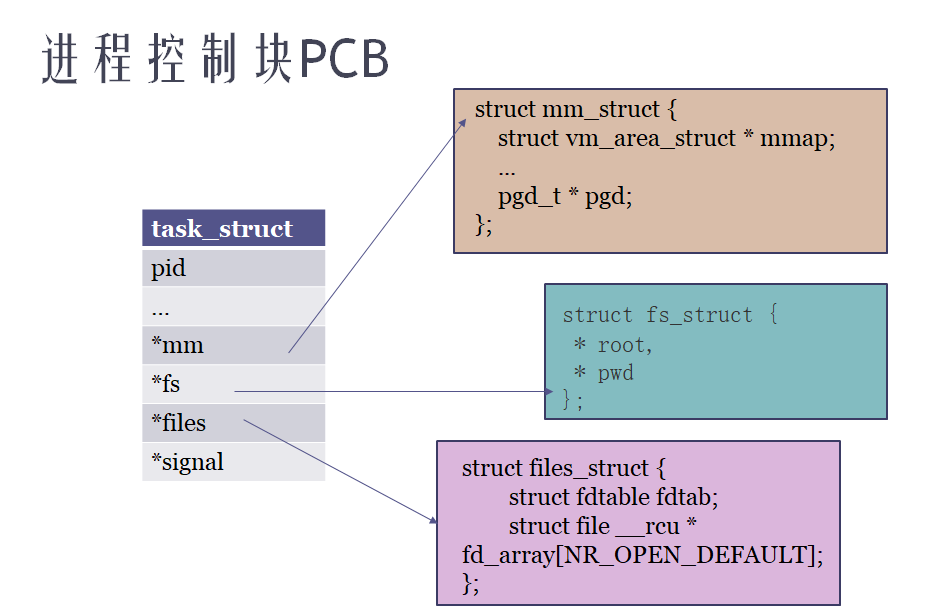
\includegraphics[width=9cm]{./figure/linux_pcb.png}
  \floatfoot{注:即linux中的task\_struct }
  }
\end{figure}
\begin{description}
  \item[\heiti{mm 内存资源:}] 进程的内存
  \item[\heiti{fs 文件系统资源1:}] 根路径和当前路径指针
  \item[\heiti{files 文件系统资源2:}] 进程打开的文件,文件描述符数组
  \item[\heiti{signal 信号资源:}] 不同进程可以针对同一信号挂不同的处理方法
  \item[\heiti{pid 属性资源:}] 描述进程的属性
\end{description}



\section{task\_struct的属性特点}
本节讲的主要是Pid属性是有限的这个特点,利用这个特点,实现linux下破坏死机和代码中破解的例子。
\subsection{fork炸弹让linux死机}
linux下著名的fork炸弹,一敲就让Linux死机。是利用不断利用fork产生进程把pid耗尽,其命令如下:
\begin{example*}
  \wdexpbox
  {\caption{fork炸弹}}
  {linux下著名的fork炸弹,一敲就让Linux死机。\\
  \textcolor[rgb]{1.00,0.00,0.00}{\#linux fork 炸弹}\\  
  \textcolor[rgb]{1.00,0.00,0.00}{\textbf{:()\{:\|:\&\};: } }
  }
\end{example*}

\begin{latexcmd}[label=linux fork 炸弹解析]
: 函数名为冒号

() 函数参数定义

{} 函数定义

:调用自己

|:递归调用自己

& 后台执行

; 函数结束

: 调用函数:
\end{latexcmd}

\subsection{pid数量限制导致安卓的一键root}
安卓的2.2.1之前的版本被发现一个漏洞,很容易就被一键root,安卓的调试软件adb刚开始时有root权限,之后adb调用api setuid(shell) 把自己从root用户降为shell用户。谷歌的工程师在调用时没有检查setuid的返回值,即默认setuid总是可以成功。黑客们利用uid数量有限制的属性,将shell用户内的pid进程全部用完,这样调用setuid时是无法成功的,但因为没有检查返回值,导致adb调用setuid(shell) 后没有降权成功,还是有root权限。这就是Android著名的提权漏洞:rageagainstthecage。2.2之后的安卓版本修复了此漏洞,方法是检查setuid的返回值。

查看Linux中最大Pid数量的命令如下:
\begin{lstlisting}[language={bash}]
wangfan@wangfan-VirtualBox:~$ ulimit -a
core file size          (blocks, -c) 0
data seg size           (kbytes, -d) unlimited
scheduling priority             (-e) 0
file size               (blocks, -f) unlimited
pending signals                 (-i) 15723
max locked memory       (kbytes, -l) 64
max memory size         (kbytes, -m) unlimited
open files                      (-n) 1024
pipe size            (512 bytes, -p) 8
POSIX message queues     (bytes, -q) 819200
real-time priority              (-r) 0
stack size              (kbytes, -s) 8192
cpu time               (seconds, -t) unlimited
max user processes              (-u) 15723
virtual memory          (kbytes, -v) unlimited
file locks                      (-x) unlimited
\end{lstlisting}

\subsection{linux的pid与tgid}
一个进程fork出子进程后,从linux内核的角度看,对应的pid肯定不一样。但是为了符合POSIX的标准要求,POSIX要求规定同一个父进程fork出的子进程,调用getpid返回的pid的号必须是一样的,我们用top命令查看进程可以看到fork出的子进程与父进程的Pid号是一样的。linux实现的原理就是通过增加一个tgid来实现父子进程调用getpid时返回值都一样的效果。
\begin{tcolorbox}[colback=blue!5,colframe=blue!75!black,title=pid和tgid 视频]
\videoattach{4- pid-tgid-pthread-self}{pid和tgid视频演示}{https://share.weiyun.com/5wYury8}
\end{tcolorbox}

\subsection{linux进程task\_struct的三种数据结构}
在linux代码中会涉及各种对task\_struct的引用关系,比如调度算法中会将task\_struct挂在链表上,父子进程的关系用树来描述,CFS调度算法会用到红黑树,通过pid查找进程则是用hash表的结构。其对应的数据结构如\ref{task_datastructure}所示

\begin{figure}[H]
 \wdfigbox
  {\caption{task\_struct汲及到的数据结构}\label{task_datastructure}}
  {
  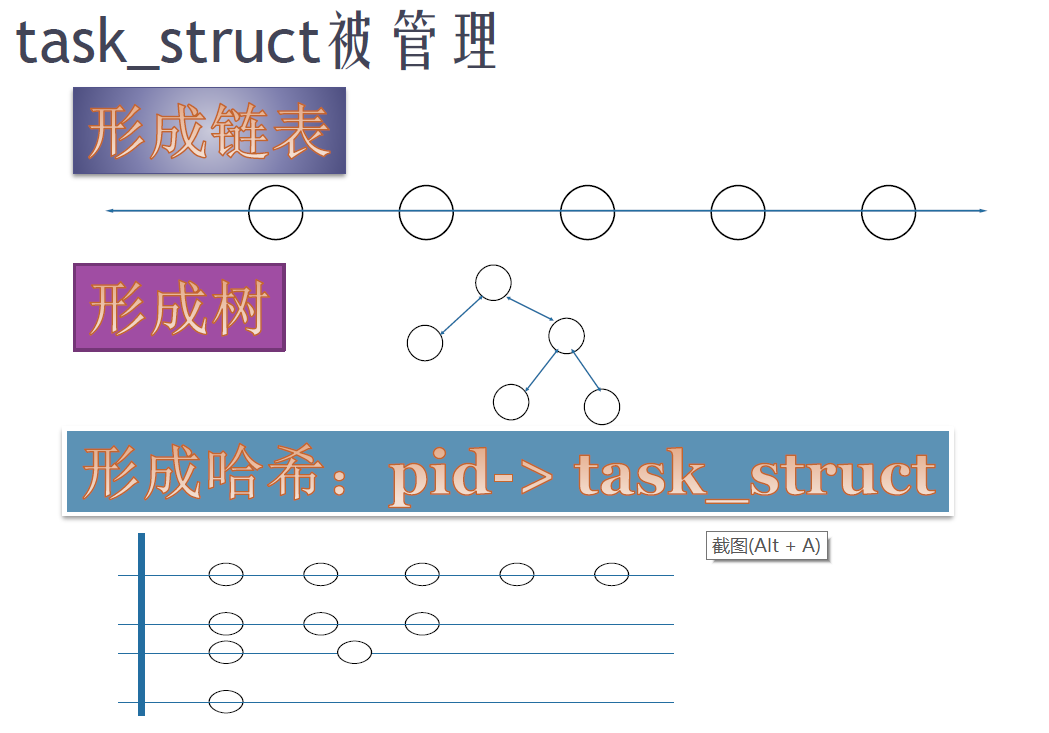
\includegraphics[width=9cm]{./figure/task_datastructure.png}
  \floatfoot{注: 每种数据结构选择都是根据应用场景的需求来选择实现目的效率最高的数据结构}
  }
\end{figure}
\chapter{进程的状态特征}
~\\linux进程的生命周期对应6个状态,
\section{进程状态切换}
\subsection{进程运行时的3个基本状态}
操作系统包括实时系统对应进程一般都有3个状态,进程在有CPU时对应运行态,无CPU时对应就绪态和睡眠态。就绪态指所有资源都准备好,只要有CPU就可以运行了。睡眠指有资源还未准备好,比如读串口数据时,数据还未发送。此时有CPU也无法运行,需要等资源准备好后变成就绪态,然后得到CPU后才能变成运行态,其转换关系如\ref{process_3types}所示。

\begin{figure}[H]
 \wdfigbox
  {\caption{进程基本的三种状态转换}\label{process_3types}}
  {
  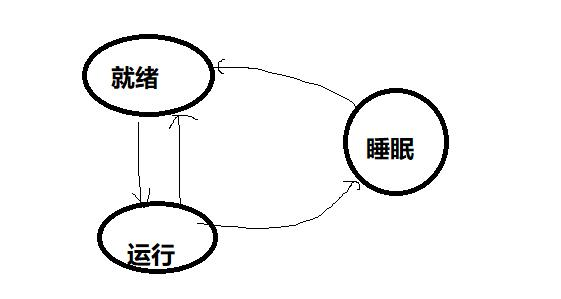
\includegraphics[width=9cm]{./figure/process_3types.jpg}
  \floatfoot{注:linux 除这三种状态外另外增加了状态}
  }
\end{figure}

\subsection{linux进程扩展的6个状态}

\begin{enumerate}
  \item {\heiti{僵尸态:}} 子进程退出后,所有资源都消失了,只剩下task\_struct,父进程在wait函数中可以得到子进程的死亡原因。在wait之前子进程的状态就是僵尸态。
  \item {\heiti{深度睡眠:}} 等待资源到位后才醒过来
  \item {\heiti{浅度睡眠:}} 等待资源到位或收到信号后都会醒过来
  \item  {\heiti{暂停:}} stop状态是被外部命令作业控制等强制进程进入的状态。
  \item  {\heiti{就绪:}} 未占用CPU,等待调度算法调度到运行态的进程
  \item  {\heiti{运行:}} 占有CPU,正在运行的线程。
\end{enumerate}

\begin{figure}[H]
 \wdfigbox
  {\caption{linux 进程6种状态转换}\label{linux_process_6types}}
  {
  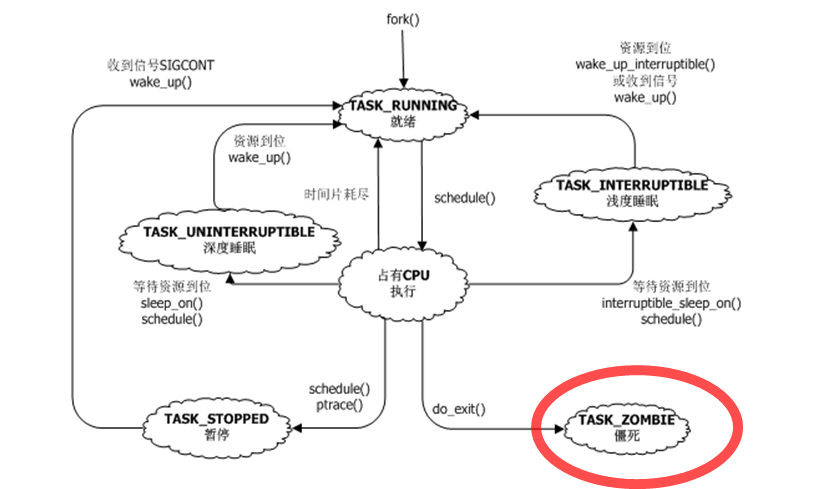
\includegraphics[width=9cm]{./figure/linux_process_6types.png}
  \floatfoot{注:linux 进程的运行转换图}
  }
\end{figure}
暂停状态是进程在运行过程中,通过外部bash命令强制让进程进入的状态。通过这种方法可以指定进程的CPU占用率。后面我们通常用cgroup的方法来实现,这里仅作了解。
\begin{latexcmd}[label=进入stop状态的方法]
作业控制的命令
ctrl + z, fg/bg
cpulimit
cpulimit -l 20 -p 10111
限制pid 为10111程序的CPU使用率不超过20%  
\end{latexcmd}
\subsection{linux进程状态的联系和区别}
\begin{description}
  \item[{\heiti{就绪VS运行}}] linux的调度算法只管理就绪和运行态中的进程,只对应\label{linux_process_6types}中的就绪和占有状态的进程,这两个状态都称为task\_running。
  \item[{\heiti{深度睡眠VS浅度睡眠}}] 深度睡眠只有资源到位才醒,收到信号也不醒,浅度睡眠资源到位或收到信号都会醒
  \item[{\heiti{睡眠VS暂停}}] 睡眠是代码中未得到资源主动进入的状态,暂停是程序外部强制进程进入的状态。
\end{description}


\section{进程的内存泄露}
内存泄露指随着时间的增长,进程的内存使用呈现线性增长的情况,指的是进程一直在运行,运行中申请了内存,但使用完后并没有释放,运行期间每次都申请内存而不释放导致系统内存越来越少的情况。这里要理解内存泄露的原因不可能是进程死了,内存没释放。因为进程死了之后就变成僵尸,Linux会自动将进程中申请的资源全部释放,只留下task\_struct让父进程wait来查看状态。不可能再占用内存。
%%% Local Variables:
%%% TeX-master: "main"
%%% End:

\partabstractfp{进程资源是如何处理的?进程与进程间是怎样的关系?进程死亡后会不会内存泄露?不同生命周期下进程资源的处理方式有什么差异?}
\partabstractrp{注:本章的架构是我根据讲课记录自己的理解划分的,可能与讲课不一致,如有错误欢迎指正。子死父收尸章节应该是第一天讲的,为了保持架构的一致性,把它挪到此处进行处理。}
\partabstractlettrine{L}{inux进程出生到死亡,生,死,睡过程} % the first word of the abstract

\part{进程课第2天}

\chapter{进程出生}
\section{进程出生时资源处理}
fork出子进程后,子进程的资源就直接从父进程的进程结构task\_struct拷贝出同样的信息,如\ref{child_fork_task_struct}所示。进程P2刚创建后,其资源是一模一样的。

\begin{figure}[H]
 \wdfigbox
  {\caption{fork子进程资源拷贝}\label{child_fork_task_struct}}
  {
  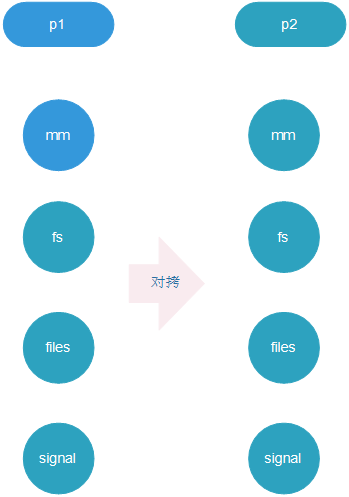
\includegraphics[width=8cm]{./figure/child_fork_task_struct.png}
  \floatfoot{注:所有资源结构体都进行拷贝  }
  }
\end{figure}
之后随着进程变化,本着谁修改谁分裂的原则进行资源变化的处理。

\section{进程分裂时的资源变化 -- COW}
父子进程刚诞生时所得到的资源是一样的,那这些资源在何时发生变化,以及变化后有什么影响,这就涉及到了linux的copy-on-write技术,下面通过 具体的实例来说明父子进程的资源变化流程。\\
COW(copy-on-write)技术是进程fork时采用的,涉及到虚拟内存和实际内存的映射关系。采用了COW技术后,进程处理会有一些现象需要重点注意。比如fork之后的父子进程读写同一个全局变量时,一个变量在不同的进程会显示出不同的值。
\subsection{COW 现象代码}
\begin{lstlisting}[language={C}]
#include <stdio.h>
#include <sys/types.h>
#include <unistd.h>
int data = 10;
int child_process()
{
    printf("child process %d, data %d\n", getpid(), data);
    data = 20;
    printf("child process %d, data %d\n", getpid(), data);
    _exit(0);
}
int main(int argc, char * argv[])
{
    int pid;
    pid = fork();
    if(pid == 0){
        child_process();
    }
    else{
        sleep(1);
        printf("parent process %d, data %d", getpid(),data);
        _exit(0);
    }
    return 0;
}
\end{lstlisting}
在正常情况下,程序修改全局变量data,再打印data,会是修改后的值 20,代码中子进程修改全局变量为20后,父进程等待1s,确保子进程已修改完成,但父进程最终打印的结果还是10。
\begin{latexcmd}[label= COW现象]
#运行程序的显示结果如下
child process 9491, data 10
child process 9491, data 20
parent process 9490, data 10
\end{latexcmd}

下面我们具体分析程序背后采用COW的原理和流程。\\
\subsection{COW 实现技术原理}
fork进程前后的内存关系如\ref{linux_fork_mem_compare}所示,
\begin{description}
  \item[\heiti{fork前第1阶段:}] 全局变量data对应数据段内存vir和phy都在数据段,权限为可读可写。
  \item[\heiti{fork后:}] vir和Phy的权限全部变成只读权限,读内存正常,写内存会进入page fault缺页中断。
  \item[\heiti{fork后写内存:}] 写内存后,发生缺页中断,Linux会重新申请一个4k内存,将新物理内存指向更改了内存地址的进程vir。同时将老的4k内存拷贝给新的内存,同时将权限改为R+W,这样父子进程的同一个vir虚拟地址就分别对应2个独立的可读可写的物理地址。总之谁先写谁拿到新的物理内存,原内存留给剩下的进程。
\end{description}
\begin{figure}[H]
 \wdfigbox
  {\caption{fork进程前后内存映射关系}\label{linux_fork_mem_compare}}
  {
  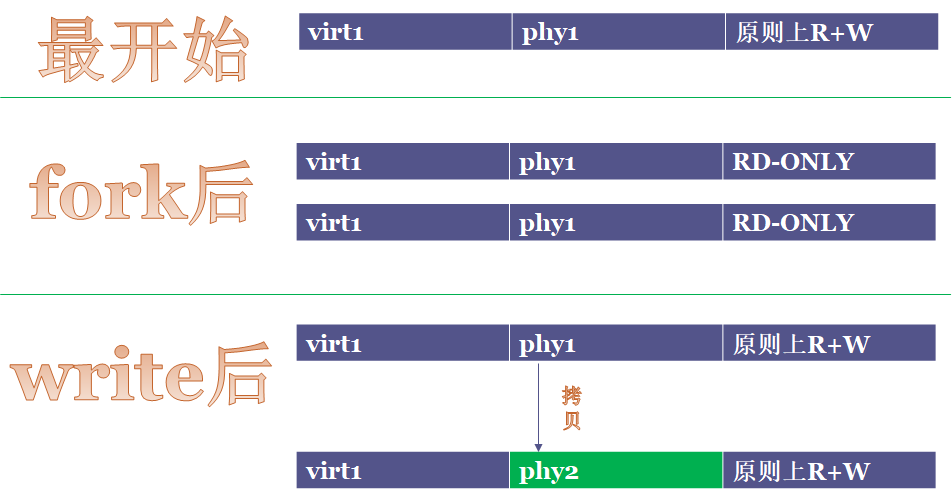
\includegraphics[width=9cm]{./figure/cow_fork_virmem_compare.png}
  \floatfoot{注:第一列为虚拟地址,第二列为物理地址,最后一列对应内存的读写权限 }
  }
\end{figure}
\subsection{无法用COW的情况:VFORK}
COW技术必须借助MMU(内存管理单元)来实现。COW是通过改变虚拟内存和物理内存的映射关系来实现,没有MMU的系统,无法实现虚拟内存和物理内存的映射。也无法调用fork函数,无MMU系统对应调用的是vfork函数,其资源变化对比fork如\ref{vfork_mem}所示:
\begin{figure}[H]
 \wdfigbox
  {\caption{vfork进程内存}\label{vfork_mem}}
  {
  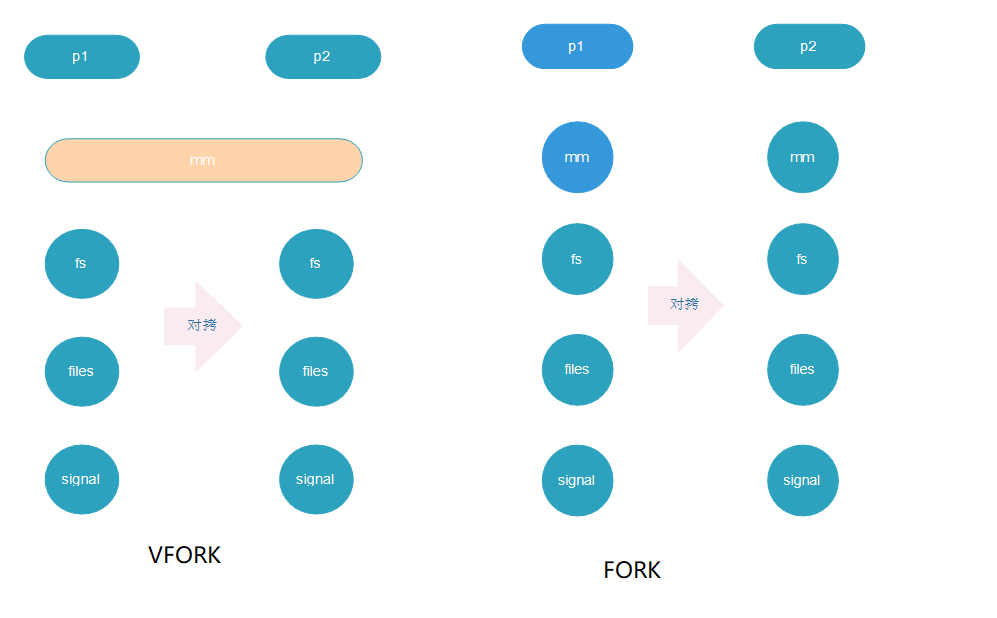
\includegraphics[width=10cm]{./figure/vfork_mem.png}
  \floatfoot{注:mm为同一份,没有进行拷贝  }
  }
\end{figure}
vfork的特点:vfork会阻塞父进程,只有等子进程完全退出后才执行父进程。vfork特性演示视频如下所示:

\begin{tcolorbox}[colback=blue!5,colframe=blue!75!black,title=vfork 视频]
\videoattach{2- vfork.avi}{vfork与COW区别}{https://share.weiyun.com/5G2jlaC}
\end{tcolorbox}

\subsection{强制共享资源--线程}
当P1和P2都用同一个资源,资源结构体不进行拷贝,P2的资源指针直接指向P1,这样就体现出线程的特征:可以调度又共享一样的资源。Linux中也是这样来实现线程的,调用pthread\_create时,会调到CLONE的API,这样就会让P2的资源指针指向P1。
\begin{figure}[H]
 \wdfigbox
  {\caption{线程资源处理}\label{thread_mem}}
  {
  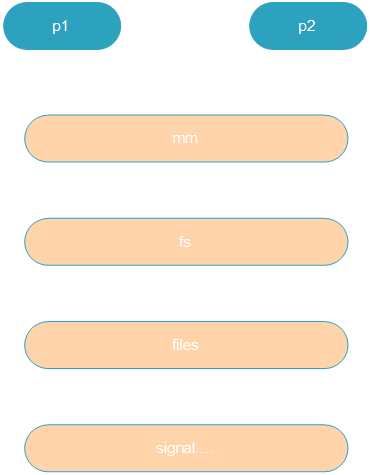
\includegraphics[width=4cm]{./figure/thread_resource.png}
  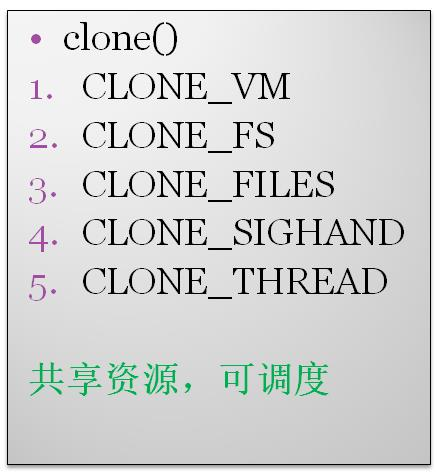
\includegraphics[width=4cm]{./figure/clone_api.jpg}
  \floatfoot{注:最终调用的API为CLONE,pthread\_create  }
  }
\end{figure}
\begin{tcolorbox}[colback=blue!5,colframe=blue!75!black,title=thread 视频]
\videoattach{3- thread.avi}{thread视频演示}{https://share.weiyun.com/5EsHhl5}
\end{tcolorbox}

\section{第1个进程,进程0与进程1}
开机后进程0创建出进程1,开机后进程0会退化成idle进程,idle进程的优先级最低。此进程运行的原则是所有其他的进程不运行时它就开始运行,当运行idle进程时,cpu就设置成低功耗模式。(注:与开机键中的suspend的区别是idle状态时只有cpu是低耗,suspend时显示器电源等其他设备也会进入低功耗)。此设计的精妙之处在于,如果不用进程0,进程进入低功耗模式的判断标准就变成了所有进程退出后要检查一下是否是最后一个进程,如果是最后一个就进入低功耗模式。这样的设计就会把检查状态耦合到了每个进程之中。增加进程0设计的好处在于,设计就简化只要判断是否在idle进程就可以了。实现了去耦合。
视频演示如下:
\begin{tcolorbox}[colback=blue!5,colframe=blue!75!black,title=idle进程视频]
\videoattach{7- idle-process.avi}{idle进程视频演示}{https://share.weiyun.com/5et9Oz8}
\end{tcolorbox}

\chapter{进程运行}
~\\程序运行时大部分进程状态为运行或睡眠。调度算法解决可以跑的运行状态(就绪和运行),剩下的不可以跑的进程就是睡眠和等待。睡眠实现对应的代码就是调用了schdule函数,唤醒则是对应的是schdule返回。一个进程等资源就会去睡,linux所有的睡眠,对应的task\_struct就会挂在队列wait\_queue上,当资源来了后,就会唤醒等待队列上的进程。视频演示如下:
\begin{tcolorbox}[colback=blue!5,colframe=blue!75!black,title=等待队列视频]
\videoattach{6- sleep-waitqueue.avi}{进程等待队列视频演示}{https://share.weiyun.com/53SMfMt}
\end{tcolorbox}


\chapter{进程死亡}
fork执行后,就会变成2个进程返回,而不是一个进程返回两次。两个进程用的是同一段代码,不同的是在判断fork的返回值后会走向不同的分支。子进程返回的是0,则if(pid == 0)后执行的是子进程,父进程接收到的返回值是子进程的pid值。如下所示:

\dirtree{%
.1 fork之后.
.2 返回值为-1\DTcomment{fork失败}.
.2 返回值为0\DTcomment{子进程返回}.
.2 返回值为pid号\DTcomment{父进程返回}.
}

\section{子死父收尸}
linux中子进程死亡时首先变成僵尸,父进程通过wait来获取子进程的死亡原因。调用的API如\ref{child_wait}所示,父进程通过分析子进程的退出码就可以知道具体的退出原因了。

\begin{figure}[H]
 \wdfigbox
  {\caption{子进程死亡原因获取}\label{child_wait}}
  {
  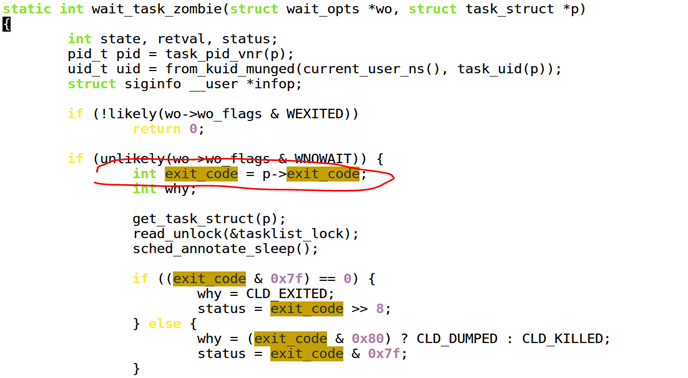
\includegraphics[width=10cm]{./figure/child_wait.png}
  \floatfoot{父进程通过exit\_code获取子进程退出信息}
  }
\end{figure}

\begin{tcolorbox}[colback=blue!5,colframe=blue!75!black,title=子进程死亡原因获取视频]
\videoattach{1- child-waited-by-parent.avi}{父进程获取子进程死亡原因视频演示}{https://share.weiyun.com/5FwLvlt}
\end{tcolorbox}
\section{父死子托孤}
任何一个进程死亡后有个原则,首先托付给subreaper,如果没有subreaper则托付给init。如\ref{child_process_died}所示。进程可以通过API来设置自己为subreaper。subreaper要注意调用wait来处理可能托付过来的僵尸进程。
\begin{figure}[H]
 \wdfigbox
  {\caption{进程死亡后挂接关系}\label{child_process_died}}
  {
  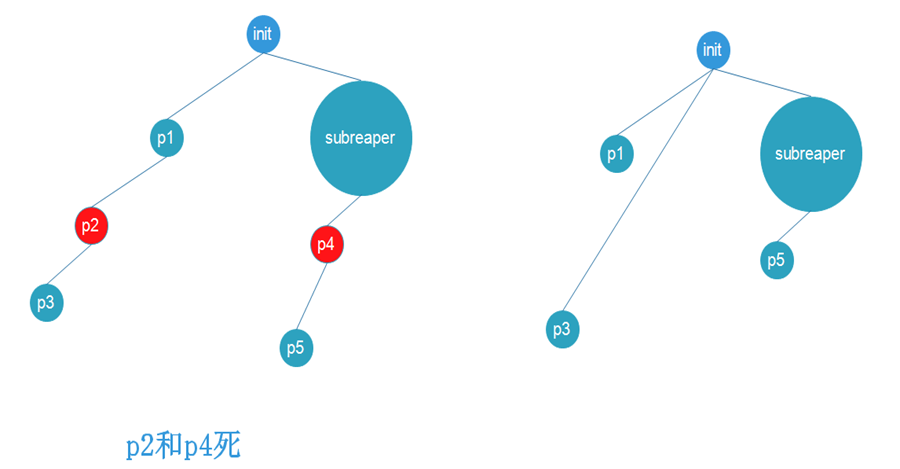
\includegraphics[width=10cm]{./figure/child_process_died.png}
  \floatfoot{挂到init或subreaper  }
  }  
\end{figure}

\begin{tcolorbox}[colback=blue!5,colframe=blue!75!black,title=进程托孤视频]
\videoattach{5- orphan.avi}{进程托孤视频演示}{https://share.weiyun.com/57CLGS4}
\end{tcolorbox}
\clearpage
%%% Local Variables:
%%% TeX-master: "main"
%%% End:


\partabstractfp{本章讲述如何根据不同类型的进程分配不同策略的调度算法,调度算法的原理及应用对象,如何更改进程的调度策略。
}
\partabstractrp{练习题:\\
\small{1. 运行2个高CPU利用率进程,调整他们的nice。\\2. 用chrt把一个死循环进程调整为SCHED\_FIFO。\\3. 阅读ARM的big.LITTLE架构资料,\\并论述为什么ARM要这么做。}}
\partabstractlettrine{L}{inux进程的类型不同,策略不同。} % the first word of the abstract

\part{进程课第3天}


\chapter{进程分类}


\section{CPU消耗与IO消耗型}
CPU消耗型是指CPU占用率高的应用,比如编译代码。IO消耗型指像读硬盘之类的应用,大部分时间消耗在DMA上,CPU占用率比较低。典型的操作系统内,IO消耗型的优先级比较高。因为IO消耗型应用往往与用户体验密切相关,比如读写硬盘和外设之类的操作,用户操作键盘和鼠标时如果长时间没有反应,就会导致体验很差。而CPU消耗型,比如编译程序,我们可以把它的优先级降低,编译时间从10分钟变成11分钟,对用户的体验影响不是很大。

IO型对CPU的强弱不敏感,对何时抢到CPU敏感。因为处理时间多数花费在非CPU的计算上,CPU处理占用的比例很小,因此CPU的强弱对IO消耗影响不大。

\section{应用:arm大小核设计}
从用户体验上,CPU运算能力越快越好,但CPU能力越强,功耗也越大。为了实现处理相同任务花费的时间和功耗更低的目标,arm采用了大核加小核的设计模式。大核CPU运算力强,功耗高,小核CPU运算力弱,功耗低。CPU调度算法根据CPU消耗型和IO消耗型的特点来分配任务到不同的核上来实现低功耗和高性能的目标。
\begin{example*}
  \wdexpbox
  {\caption{ARM的big.LITTLE设计}}
  {采用大核+小核的设计,大核功耗高,运算力强,用于处理CPU消耗性任务,小核功耗低,功耗小,用于处理I/O消耗性任务。实现功耗降低,但处理效果与全是大核处理一致的效果}
\end{example*}

\chapter{进程调度策略}
~\\\indent Linux调度算法的设计目标是满足2个指标:吞吐量与响应。这两个指标是矛盾的,一个指标的上升必然影响到另一个指标的性能。从用户的角度来看,吞吐量是完成所有工作负载花费时间最少,响应是指处理任务时响应时间最短。简单地说就是linux在单位时间内切换任务的次数越多,响应任务的时间越快,但由于切换任务所需的上下文开销,会导致吞吐量的下降。根据不同的应用场景,我们会选择不同的算法来达到这两个指标的平衡。

linux的进程分RT进程和NORMAL进程两种,RT进程没有nice值,执行自己的调度算法。NORMAL进程根据自己的nice值采用相应的算法进行调度。
Linux 2.6之前执行优先级与nice值相关,nice值随进程睡的时间动态相关,普通NORMAL进程的nice值执行动态变化的策略,睡得越久,优先级越高。

2.6之后增加了2个补丁:{\heiti{熔断机制补丁}}和{\heiti{CFS调度算法}}。
\begin{description}
  \item[{\heiti{1. 熔断补丁:}}] 限制了RT进程和NORMAL进程的比例,当RT进程一直占用CPU到了熔断阈值的时刻,强制调度让NORMAL进程运行。
  \item[{\heiti{2. CFS调度算法:}}] 改进了NORMAL进程的调度算法,采用红黑树实现完全公平的调度策略。
\end{description}
\clearpage


\section{RT进程调度}
Linux调度进程时主要考虑两个要素:策略和优先级。RT进程没有nice值。其调度策略分成SCHED\_FIFO和SCHED\_RR两种。S
Linux所有的优先级分成0-139,其中0-99为RT进程,100-139对应普通进程(nice值 -20到19)。数字越小优先级越高。
RT进程和普通进程的调度区别如下:
\begin{enumerate}
  \item RT进程优先级高的进程未睡眠,优先级低的进程无法抢占。
  \item 普通进程优先级低的进程也可以抢占高优先级的普通进程,区别在于抢到的CPU时间会比较少。
\end{enumerate}


对应视频如下:
\begin{tcolorbox}[colback=blue!5,colframe=blue!75!black,title=进程调度策略视频]
\videoattach{1- scheduler.avi}{linux调度算法.avi}{https://share.weiyun.com/5yQ78xI}
\end{tcolorbox}

\subsection{SCHED\_FIFO}
如果进程优先级最高,进程就会一直运行到睡眠才让出CPU。
\subsection{SCHED\_RR}
RR的含义是round-robin,CHED\_FIFO和SCHED\_RR在不同优先级上表现完全一样。区别在于同等优先级的调度上,SCHED\_FIFO策略对应的进程会一直跑到睡眠才轮转到其它同等优先级的RT进程运行。SCHED\_RR会根据时间片进行轮转。


\section{NORMAL进程调度}
\subsection{动态惩罚与奖励机制}
Linux 2.6早期版本优先级不完全取决于代码中设置的进程nice值,nice值设置之后还会对普通进程进行一个评估,其优先级是动态调整的。评估标准是睡眠越久,优先级越高。优先级是随着睡眠时间的增加而增加,占用CPU的时间越长,优先级会随着降低。此算法的缺点是进程干活越久优先级越低,会导致经常处理任务的进程优先级越来越低,干的活越来越少。之后加入的补丁引入了CFS算法修正了这个缺陷。
\subsection{CFS调度}
CFS(Completely Fair Scheduler)完合公平调度指的是保证所有NORMAL进程(task\_struct)虚拟运行时间完全相同。其虚拟运行时间的计算公式为
$$vtime = ptime * 1024 /weight $$
\noindent\textbf{ptime:} 指进程运行物理时间\\
\textbf{1024:}系数\\
\textbf{weight:} 权重,由nice值决定。\\

\begin{figure}[H]
 \wdfigbox
  {\caption{weight权重表}\label{cfs_weight}}
  {
  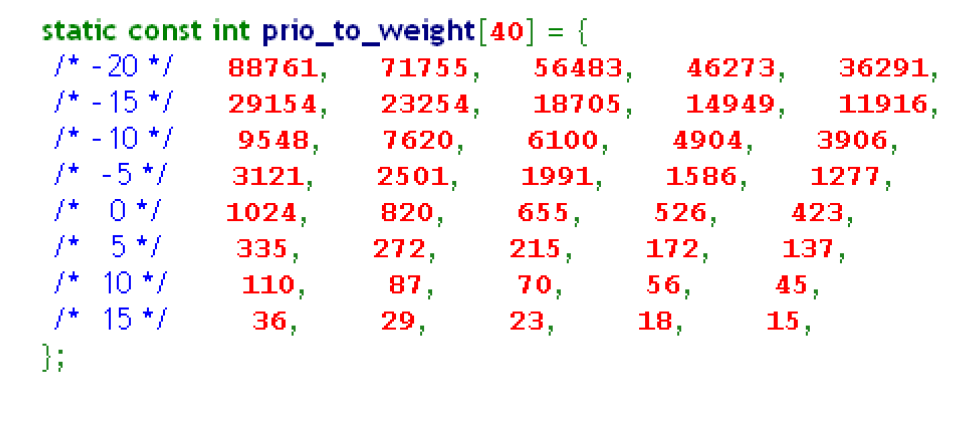
\includegraphics[width=10cm]{./figure/cfs_weight.png}
  \floatfoot{nice=0时,虚拟时间等于物理时间  }
  }
\end{figure}

所有虚拟时间挂在红黑树上,每次linux调度虚拟时间最小的进程运行。

\chapter{调整优先级}

~\\调度优先级是内核分配给进程的代表执行先后可能的整数(-20-19)
整数值越小,优先级越高。bash shell默认以优先级0来启动所有进程,可通过nice命令和renice调整。
\section{用 nice 改变进程优先级}
对于普通用户来说,只可以以更低优先级运行命令,更高优先级运行命令需要高级用户权限。
nice命令是为未运行命令指定运行时调度优先级的,如果是已运行的命令则需要renice命令
\begin{latexcmd}[label=nice命令改变进程优先级]
#以10优先级值后台运行httpd命令
nice -n 10 httpd &

-n后面整数指定httpd命令运行的优先级
httpd即要改变优先级的命令
&表示此命令为后台运行
\end{latexcmd}
\begin{tcolorbox}[colback=blue!5,colframe=blue!75!black,title=nice设置进程视频]
\videoattach{3- nice.avi}{nice设置进程.avi}{https://share.weiyun.com/50Ij0ba}
\end{tcolorbox}

\section{用 renice 改变进程优先级}

renice命令与nice命令用法一样,限制也一样(普通用户只能以更低的调度优先级运行命令),惟一不同就是可以更新正在运行命令的调度优先级。
\begin{table}[!htbp]
\stabbox{2.2cm}
{\caption{Linux renice 命令参数含义}\label{}}
{\begin{tabular*}{\cflwidth}{@{\hspace{5pt}}@{\extracolsep{\fill}}*{3}{@{\hspace{-3pt}}l}}
    \heiti{参数} &  \heiti{含义 }              \\
    %\toprule
    -g &  使用程序群组名称,修改所有隶属于该程序群组的程序的优先权。             \\
    -p &   改变该程序的优先权等级,此参数为预设值。          \\
    -u &  指定用户名称,修改所有隶属于该用户的程序的优先权。      \\
\end{tabular*}
\floatfoot*{}
}
\end{table}

\begin{latexcmd}[label=nice命令改变进程优先级]
#PID为5200的进程nice设为-5
renice -5 -p 5200
\end{latexcmd}
\begin{tcolorbox}[colback=blue!5,colframe=blue!75!black,title=renice设置进程视频]
\videoattach{2- renice.avi}{renice设置进程.avi}{https://share.weiyun.com/5kRR0lo}
\end{tcolorbox}

\section{用 chrt 改变进程优先级}
使用实时调度策略,必须具有root权限。
chrt 命令的策略选项
\begin{table}[!htbp]
\stabbox{3.0cm}
{\caption{Linux chrt 命令参数含义}\label{}}
{\begin{tabular*}{\cflwidth}{@{\hspace{5pt}}@{\extracolsep{\fill}}*{4}{@{\hspace{-3pt}}l}}
    \heiti{短选项} & \heiti{长选项 }  & \heiti{詳細 }              \\
    %\toprule
    -f & --fifo   &  调度器设成 SCHED\_FIFO              \\
    -o & --other  &   调度器设成 SCHED\_OTHER            \\
    -r & --rr     &   调度器设成 SCHED\_RR           \\
    -a & --all-tasks &  设置Pid号对应的所有线程              \\
\end{tabular*}
\floatfoot*{}
}
\end{table}

\begin{latexcmd}[label=chrt使用方法]
# 确认某个进程的属性可以通过指定 -p 或 --pid 并指定进程ID,用法如下:
# chrt -p 468
pid 468's current scheduling policy: SCHED_FIFO
pid 468's current scheduling priority: 85

# chrt -p 476
pid 476's current scheduling policy: SCHED_OTHER
pid 476's current scheduling priority: 0

# 将PID 1000 的进程设定成 SCHED_FIFO,优先级设定成50。
chrt -f -p 50 1000

# 将PID 1000 的进程设定成 SCHED_OTHER,优先级设定成0。
chrt -o -p 0 1000

# 起动 /bin/my-app 设定成 SCHED_FIFO,优先级设定成36。
chrt -f 36 /bin/my-app
\end{latexcmd}
\begin{tcolorbox}[colback=blue!5,colframe=blue!75!black,title=chrt设置进程视频]
\videoattach{4- chrt.avi}{chrt设置进程.avi}{https://share.weiyun.com/5c3Upbl}
\end{tcolorbox}


%%% Local Variables:
%%% TeX-master: "main"
%%% End:



\partabstractfp{\\这里讲的是CPU处理的负载,对应负载指CPU处理的任务。\\
1. linux的4种不同优先级任务是什么\\
2. 不同优先级任务间的抢占原则是什么?\\
3. 负载均衡的不同类型及使用方法。\\
实时性要求的应用场景\\
4. 实时系统是什么?\\
5.linux 为什么不是一个硬实时系统?\\
6.linux RT实时补丁的原理,使用方法及限制。}
\partabstractrp{练习题:\\
\small{
1. 用time命令跑一个含有两个死循环线程的进程。\\
2. 用taskset调整多线程依附的CPU。\\
3. 创建和分群CPU的cgroup,调整权重和quota\\
4. cyclictest}}
\partabstractlettrine{负}{载均衡} % the first word of the abstract

\part{进程课第4天}


\chapter{负载均衡}
\section{LINUX下的负载均衡处理对象}
负载均衡是最大化利用CPU资源的方法,要求在有任务(task\_struct,中断,软中断)执行时,所有的CPU都能利用上,不产生有任务处理却有CPU闲置的情况。首先从任务的优先级的角度来看,CPU处理的任务只有下面4种优先级,按高到低依次是:


\begin{table}[!htbp]
\stabbox{3.0cm}
{\caption{Linux CPU对应的4类不同优先级区间}\label{linux_pri_4type_table}}
{\begin{tabular*}{\cflwidth}{@{\hspace{5pt}}@{\extracolsep{\fill}}*{3}{@{\hspace{-3pt}}c}}
    \heiti{优先级 } & \heiti{Linux 中 CPU所处状态   }              \\
    %\toprule
    1 & 中断                 \\
    2 & 软中断                  \\
    3 & 处于spinlock等关闭了调度区间的进程                   \\
    4 & 普通进程                  \\
\end{tabular*}
\floatfoot*{附注: 优先级数字越低优先级越高:中断 > 软中断  > spinlock > 普通进程}
}
\end{table}
以上优先级的任务在linux处理规则如下:

\begin{enumerate}
  \item 中断不可以嵌套中断,在2.6版本后,处于中断区间再次发生中断时,会等到前一个中断执行结束后再进行处理下一个中断。
  \item 中断可以唤起软中断
  \item 软中断可以唤起中断
  \item CFS等调度算法只处理普通进程和普通进程之间的调度,不涉及中断,软中断,及关闭了调度的进程。具体表现如下:\begin{itemize}
        \item 如果CPU在处理1,2,3优先级的任务时,不受调度算法的调度,只有等处理完1,2,3优先级的任务后才会再由调度算法调度。
        \item 如果CPU在处理4普通进程的任务时,高优先级的中断和软中断可以直接抢占普通进程,不用等调度算法调度。
        \end{itemize}
\end{enumerate}
\section{中断负载均衡}
在TOP命令中,cpu时间占用中有一列是\textbf{hi}和\textbf{si},分别对应中断和软中断。说明cpu时间除了在task\_struct上,还有可能花在中断和软中断,当网络流量比较大时,cpu花在中断和软中断的时间比较大,可以考虑中断负载均衡。\\

分配IRQ到某个CPU,掩码01代表CPU0,02代表CPU1,04代表CPU2,08代表CPU3



\begin{latexcmd}[label= 中断分配到CPU方法]
#此命令将中断145分配到CPU0上处理
[root@boss ~] # echo 01 > /proc/irq/145/smp_affinity
[root@boss ~] # cat /proc/irq/145/smp_affinity
			00000001
\end{latexcmd}
\section{软中断负载均衡--rps}
有时候有的网卡只有一个队列,一个队列的中断只能分配到一个核,Linux设计是一个核上抛出的软中断只能在同一个核上执行,cpu 0上的中断抛出一个软中断,tcp/ip协议栈也只能在cpu 0的软中断上处理。google在linux内核里面加入了rps补丁,其作用是尽管中断是在一个cpu核上,但tcp/ip协议处理的软中断可以在多个核上进行处理。rps的原理是收到软中断后通过核间中断的方法给另外的核发中断,让其他核处理软中断,从而支持单队列情况下的网络负载均衡。
\begin{latexcmd}[label= rps 使能方法]
  #rps 使能方法,除了CPU 0 外都参与TCP/IP协议栈
echo fffe > /sys/class/net/eth1/queues/rx-0/rps_cpus

#查看softirqs
wangfan@wangfan-VirtualBox:~$ cat /proc/softirqs
                    CPU0       CPU1
          HI:          0          2
       TIMER:    6841572    6725135
      NET_TX:          1      17644
      NET_RX:        679     224896
       BLOCK:      61380     180153
    IRQ_POLL:          0          0
     TASKLET:         15       7834
       SCHED:    3148547    3016778
     HRTIMER:          0          0
         RCU:     747890     885505
\end{latexcmd}
\clearpage
\begin{example*}
  \wdexpbox
  {\caption{利用rps解决cpu占用率高的问题}}
  {宋老师关于爱立信工程师的问题处理,爱立信的工程师在服务器上写了个软件发现16核有2个核占用率很高,但其他核都很闲,top命令查看发现\textbf{hi}和\textbf{si}很高,说明cpu大部分时间在处理中断和软中断,而不是处理task\_struct。解决方法是登录机器后敲命令echo ffff 到rps,cpu占用率降了下来,效果很明显。}
\end{example*}

\section{进程间(task\_struct)负载均衡}
\subsection{linux负载均衡算法原则}
linux下所有CPU核会进行分布式的PUSH和PULL操作,当CPU核空闲时会向周围的核PULL任务来执行,CPU核本身在执行任务时也会PUSH任务到其他核。
每个核执行同样的负载均衡算法,负载均衡包括RT任务的负载均衡和普通任务的负载均衡。

RT任务的负载均衡 算法是将N个优先级最高的RT分布到N个核。

\verb|pull_rt_task(); push_rt_task()|

普通任务负载均衡有三种:IDLE式负载均衡,周期性负载均衡,FORK和EXEC式负载均衡

\begin{description}
  \item[\heiti{1 周期性负载均衡:}] 时钟tick的时间点上CPU核查询自己是否很闲,周围核是否很忙,是则用PULL将周围核的任务拉过来处理。
  \item[\heiti{2 IDLE式负载均衡:}] 当CPU核在IDLE时会查询周围核是否在忙,如果旁边核比较忙时,自动PULL旁边核的task\_struct任务来执行。
  \item[\heiti{3 FORK和EXEC式负载均衡:}] FORK和EXEC创建一个新的进程时,Linux会自动找一个最闲的核将FORK和EXEC新创建出的进程放在上面处理。
\end{description}
以上处理由核与核之间分布式负载均衡处理是自动进行的。

\begin{example*}
  \wdexpbox
  {\caption{cpu占用率200\%的原因}}
  {在一个程序中起2个进程,每个进程都在做CPU消耗型操作(代码中调用while(1)死循环),在进程执行的过程中会自动将进程分配到2个CPU核上进行处理。可以通过查看CPU占用率和时间占用情况来验证。分配到两个CPU核后,CPU占用率会上升到200\%,用time计算程序的占用时间,真实时间是系统时间的一半,因为系统时间是单独统计每个CPU核上占用的时间,2个CPU核上会统计2次,显示的结果就是系统时间是真实时间的2倍。}
\end{example*}

\subsection{设置进程在指定CPU上运行}
要设置进程在指定CPU上运行,在代码里可以通过调用相关API实现,也可以直接在BASH中通过taskset命令实现。
\begin{lstlisting}[language={C}]
//设置CPU task affinity api
#include<pthread.h> //注意<pthread.h>包含<sched.h>
int pthread_setaffinity_np(pthread_t thread,size_t cpusetsize,const cpu_set_t *cpuset);
int pthread_getaffinity_np(pthread_t thread,size_t cpusetsize, cpu_set_t *cpuset);
int sched_setaffinity(pid_t pid, size_t cpusetsize, cpu_set_t *mask);
int sched_getaffinity(pid_t pid, size_t cpusetsize, cpu_set_t *mask);
\end{lstlisting}

\begin{lstlisting}[language={bash}]
# taskset在bash下的使用方法
# 命令行形式设置CPU亲核性
taskset [options] mask command [arg]...
taskset [options] -p [mask] pid

PARAMETER
    mask : cpu亲和性,当没有-c选项时, 其值前无论有没有0x标记都是16进制的,
        当有-c选项时,其值是十进制的.
    command : 命令或者可执行程序
    arg : command的参数
    pid : 进程ID,可以通过ps/top/pidof等命令获取


OPTIONS
    -a, --all-tasks (旧版本中没有这个选项)
        这个选项涉及到了linux中TID的概念,他会将一个进程中所有的TID
             都执行一次CPU亲和性设置.
        TID就是Thread ID,他和POSIX中pthread_t表示的线程ID
             完全不是同一个东西.
        Linux中的POSIX线程库实现的线程其实也是一个进程(LWP),
             这个TID就是这个线程的真实PID.
       -p, --pid
              操作已存在的PID,而不是加载一个新的程序
       -c, --cpu-list
              声明CPU的亲和力使用数字表示而不是用位掩码表示. 例如 0,5,7,9-11.
       -h, --help
              display usage information and exit
       -V, --version
              output version information and exit
USAGE

    1) 使用指定的CPU亲和性运行一个新程序
      taskset [-c] mask command [arg]...
        举例:使用CPU0运行ls命令显示/etc/init.d下的所有内容
          taskset -c 0 ls -al /etc/init.d/

    2) 显示已经运行的进程的CPU亲和性
      taskset -p pid
        举例:查看init进程(PID=1)的CPU亲和性
          taskset -p 1

    3) 改变已经运行进程的CPU亲和力
        taskset -p[c] mask pid
     举例:打开2个终端,在第一个终端运行top命令,第二个终端中
     首先运行:[~]# ps -eo pid,args,psr | grep top #获取top命令的pid和其所运行的CPU号
     其次运行:[~]# taskset -cp 新的CPU号 pid       #更改top命令运行的CPU号
     最后运行:[~]# ps -eo pid,args,psr | grep top #查看是否更改成功

PERMISSIONS
        一个用户要设定一个进程的CPU亲和性,如果目标进程是该用户的,则可以设置,
        如果是其他用户的,则会设置失败,提示 Operation not permitted.
        当然root用户没有任何限制.
        任何用户都可以获取任意一个进程的CPU亲和性.
\end{lstlisting}
\subsection{给进程指定比例的CPU负载--cgroup}
当前的程序是按程序的需要来占用cpu的,这样可能会出现一些问题,比如用户A和B在同一个服务器上,如果A开的线程比B多,可能导致A一直占用cpu,B因为线程少,占用的权重比例少而得不到cpu。于是我们想要一个分群的概率,让A和B各占有50\%的CPU,不管A线程有多少,最多只能占50\%的CPU,这样保证B即使线程数量少,也可以得到足够的CPU来运行。同样的道理类似于计费的网络带宽,可以根据用户缴费的情况分配CPU,如果未交费,就算CPU空闲也不分配CPU给用户。

\textbf{cgroup使用方法}
cgroup主要是设置以下3个属性,在\fbox{/sys/fs/cgroup/cpu}目录mkdir一个group后,会出现很多属性文件,我们主要通过以下属性来查询和设置。

\begin{description}
  \item[\textbf{cgroup.procs:}] 将进程号echo进去
  \item[\textbf{cpu.cfs\_period\_us:}] 默认是100000 基准时间100ms
  \item[\textbf{cpu.cfs\_quota\_us:}] 配额默认是-1最大值,设置可以比100000大,它与period的比例表示gruop内线程最高可占cpu的比例
  \item[\textbf{cpu.shares:}] 权重,默认是1024,调节cpu.shares可以调节不同group的cpu占用率
\end{description}

\begin{latexcmd}[label= cgroup 操作方法]
# 1 cd /sys/fs/cgroup/cpu 目录创建不同的group
# 2 mkdir A  创建 group A
# 3 mkdir B  创建 group B
# 4 /sys/fs/cgroup/cpu/A  echo 3582 > cgroup.procs 将进程3582加入A group
# 5 /sys/fs/cgroup/cpu/B  echo 3581 > cgroup.procs 将进程3581加入B group
# 6 /sys/fs/cgroup/cpu/A  echo 50000 > cpu.cfs_quota_us
    设置A group 权重为 50% cpu,  A内线程的cpu占用率最高不超过50%
\end{latexcmd}


\begin{example*}
  \wdexpbox
  {\caption{安卓的cgroup设计}}
  {安卓5.0之后的版本用到了cgroup,安卓早期版本所有进程都采用调度算法公平调度,最新版本把进程分为前台交互进程和后台非交互进程,前台的权重是1024,后台的权重是52,这样前台可以得到更多的CPU,用于提高前台程序的响应。}
\end{example*}


\chapter{实时系统}
\section{Real Time 实时系统的含义}
实时不是越快越好,是指可预期性。比如发射导弹时,必须保证在截止期限内发射出去,否则后果可能是灾难性的。硬实时强调在恶劣的情况下,从唤醒到任务真正执行之间的时间是可预期的,可以保证在预期的时间内执行到。Linux设计不保证是可预期的,因为Linux在中断,软中断,及spinlock的区间时是不可抢占的,这些区间内的执行时间是不可预期的。linux不是硬实时的系统,是软实时。
\section{抢占:Linux无法硬实时的原因}
要实现实时,最重要的就是要实现任何时刻都可以在预定期限内实现进程抢占,来保证进程可以在预期内执行。Linux无法硬实时的原因就是Linux的CPU在的4类区间有3类是无法进行抢占的,如果CPU进入了这3类区间,Linux是无法保证在这3类区间内的运行时间的。所以无法达到硬实时的要求。\\Linux
抢占的时机很多,我们主要记住不可抢占的时机:1、中断,2、软中断,3、spinlock区间的进程。
如果在这三类任务时间内唤起了高优先级的任务,任务是不能抢占的,只有当CPU脱离了这三类区间后,高优先级的任务才可以进行抢占。
如\ref{linux_pri_4type_table}所示,如果在一二三类区间唤醒了高优先级的进程,当前无法进行抢占,只有当CPU退回到第4类普通进程区间时才开始抢占。
%\begin{figure}[H]
%  \centering
%  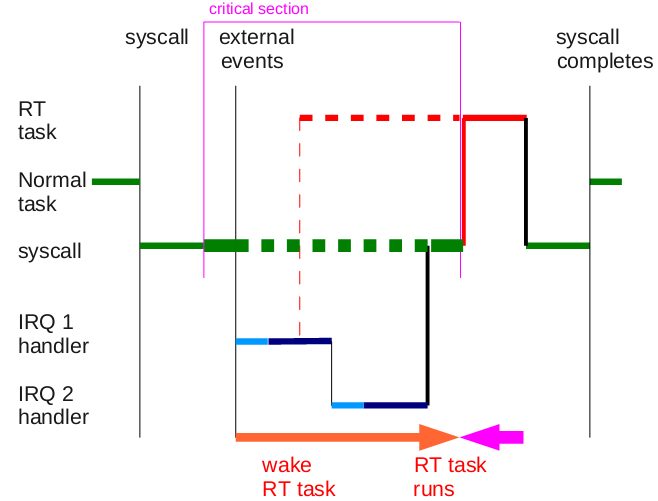
\includegraphics[width=12cm]{./figure/linux_rt_4type_preempt.png}
%  \caption{Linux的4类抢占区间}\label{linux_rt_4type_preempt}
%\end{figure}

\section{Linux实时补丁的用法}
linux的RT版本,https://wiki.linuxfoundation.org/realtime/start 这个项目是实现Linux的实时版本。主要原理是将Linux的中断线程化,即把一二三类区间都转换成四类区间。相应的linux 源码RT版本只针对特定的几个版本,使用方法是将代码中的RT补丁merge到对应的源码中,linux的RT可以做到100us量级的实时性能,(vxworks是几个us),相应的吞吐性能也会下降。

安装linux的调度器的抢占模型选项
\begin{enumerate}
  \item server版本 (不抢占)
  \item desktop版本 (kernel 内不抢占)
  \item no-latency desktop (kernel 内可抢占,手机桌面一般用此模型)
  \item completely preemption (kernel 内一二三类中断软中断都可抢占)
\end{enumerate}


安装RT补丁后还是会有很多的代码坑需要处理,比如内存管理方面,Linux的内存分配是LAZY式,当用到时才实际分配,安装实时补丁后有可能出现写内存时内存实际还未分配的情形。
\begin{tcolorbox}[colback=blue!5,colframe=blue!75!black,title=Linux无法实时的原因视频]
\videoattach{6- why-not-rt.avi}{Linux无法硬实时的原因.avi}{https://share.weiyun.com/5uPnnwZ}
\end{tcolorbox}
 
 
\begin{example*}
  \wdexpbox
  {\caption{单反上的实时系统应用}}
  {实时系统的另一个应用场景是安装2个系统:实时系统和Linux,比如单反之前用的都是实时操作系统,现在为了增加蓝牙,wifi等功能,用一个核执行实时系统,另一个核用Linux来实现蓝牙等功能}
\end{example*}

%%% Local Variables:
%%% TeX-master: "main"
%%% End:

\partabstractfp{}
\partabstractrp{}
\partabstractlettrine{F}{AQ,本章记录课间和课后宋老师以及同学们答疑} % the first word of the abstract

\part{进程问题集锦}

\chapter{课后答疑}


~\\以下问题为宋老师在微信答疑群中回答记录,微信群问题不定期提出,此部分内容会随之更新。
\begin{enumerate}
  \item
\begin{tcolorbox}[colback=green!5,colframe=green!75!black]
\heiti{Q: rps后,非多队列网卡,中断会再给每个核发中断来派发软中断?}
\tcblower
A: 中断只发一个core,这个core自己给别的core发核间中断
\end{tcolorbox}

  \item
\begin{tcolorbox}[colback=green!5,colframe=green!75!black]
\heiti{Q: rt补丁,是不是只有RT\_FULL支持优先级反转?}
\tcblower
A: 不是,不需要rt补丁就支持优先级继承,早就Merge到了mainline。\\
不叫支持优先级反转,反转是个问题,继承是解决它的方法。反转是个现象,不存在支持不支持。\\
你的问题是错误的。
\end{tcolorbox}


  \item
\begin{tcolorbox}[colback=green!5,colframe=green!75!black]
\heiti{Q: 所以softirq的优先级都是相同的吗?}
\tcblower
A: 不是的,它是一个bit的设置,检查哪个bit被设置,肯定是有先后顺序。挨个检查哪个bit的。不过这个不是关键点。你关心延迟的实时性的时候,你根本就消灭了softirq.
\end{tcolorbox}

  \item
\begin{tcolorbox}[colback=green!5,colframe=green!75!black]
\heiti{Q: 内核管理多核好理解,但内核如何管理多CPU?}
\tcblower
A: 异构多os和Linux没关系,那是多os之间的问题,不是Linux管理范畴,几个OS一个通信方法即可。
\end{tcolorbox}

  \item
\begin{tcolorbox}[colback=green!5,colframe=green!75!black]
\heiti{Q: cfs调度单位是task\_struct,那像HMP EAS这些调度器单位是什么?}
\tcblower
A: 调度单元与调度算法无关,你说的调度器和我们说的调度器不一定是一个意思。调度单元就算线程。这个不以任何操作系统,任何算法为转移。
\end{tcolorbox}


  \item
\begin{tcolorbox}[colback=green!5,colframe=green!75!black]
\heiti{Q: 课上说多核可以运行rtos+linux,那是不是单核各自运行一个OS,如何实现,是启动linux后,再启动rtos运行到某个核吗 ?}
\tcblower
A: 多个core单独各玩各的,谁先启动没有讲究,取决于产品,这个和linux没有关系,两个CPU各自运行自己的一套软件。你直接想象成两个电脑就好了。
\end{tcolorbox}



  \item
\begin{tcolorbox}[colback=green!5,colframe=green!75!black]
\heiti{Q: rt的Linux如何对付内存的lazy问题?能否改用内核的api解决用户态内存申请的实时性问题。}
\tcblower
A: 内核和用户态都是用相同的算法来进行调度,内核的调度没有比用户态更优越,用户态的调度策略和优先级比内核高时也可以抢占内核的。内存方面lazy有它的解法,主要是先申请malloc,立即释放,稳住堆;提前调用一个很大的临时变量的函数,稳住栈;提前把线程都创建;mlockall屏蔽交换。这些都有套路,看文档即可。
\end{tcolorbox}



  \item
\begin{tcolorbox}[colback=green!5,colframe=green!75!black]
\hei{Q: 有人说一但调用了\_\_do\_softirq,这个函数不可抢占,这种说法是否正确?}
\tcblower
A: 该怎么抢怎么抢,该抢的你让它抢,你只需保证抢了后的数据不出错即可。别的核还是可以访问你的核正在访问的数据的,tasklet里面该加的锁就得加。保护数据而不是保护过程。
\end{tcolorbox}
\end{enumerate}

%%% Local Variables:
%%% TeX-master: "main"
%%% End:



\partabstractfp{}
\partabstractrp{参考的文件以PDF附件的形式,可以双击链接打开或保存,需选择支持PDF附件的PDF阅读器,建议使用adobe的阅读器打开附件}
\partabstractlettrine{参}{考这章列举了用到的相关资料源地址} % the first word of the abstract
\part{参考资料}
\chapter{参考文献}
\section{宋宝华相关网站资源}
\begin{enumerate}
  \item \href{https://edu.csdn.net/course/detail/5995}{CSDN视频课程 打通Linux脉络系列:进程、线程和调度}
  \item linux公众号:\textbf{Linux阅码场}
\end{enumerate}

\section{相关文章网址}
\begin{enumerate}
  \item \href{https://blog.csdn.net/feglass/article/details/46403501}{Android提权漏洞分析——rageagainstthecage}
  \item \href{https://github.com/21cnbao/training/blob/master/kernel/drivers/globalfifo/ch12/globalfifo.c}{globalfifo.c github源码地址}
  \item 
\end{enumerate}

\chapter{相关附件}
\section{pdf课件}
\ifattachpdffile
4天课程的PPT讲义,请用支持PDF附件的阅读器打开本文档,双击打开附件或在附件中另存为处理。
\else
4天课程的PPT讲义,链接在腾讯微云上。
\fi
\begin{enumerate}
  \item \videoattach{process_schedule_lesson1.pdf}{第1天进程讲义PDF}{https://share.weiyun.com/5PZzSJk}
  \item \videoattach{process_schedule_lesson2.pdf}{第2天进程讲义PDF}{https://share.weiyun.com/5X3kLcZ}
  \item \videoattach{process_schedule_lesson3.pdf}{第3天进程讲义PDF}{https://share.weiyun.com/5vuY8Jw}
  \item \videoattach{process_schedule_lesson4.pdf}{第4天进程讲义PDF}{https://share.weiyun.com/5CiC3Ew}
\end{enumerate}



\section{视频文件}
\ifattachpdffile
4天课程的所有的视频文件,请用支持PDF附件的阅读器打开本文档,双击打开附件或在附件中另存为处理。
\fi
\subsection{第一天视频文件}
\begin{enumerate}
  \item \videoattach{1- child-waited-by-parent.avi}{父进程获取子进程死亡原因.avi}{https://share.weiyun.com/5H21I1y}
  \item \videoattach{2- zombie.avi}{子进程变成僵尸.avi}{https://share.weiyun.com/5kkIww6}
  \item \videoattach{3- stop-status.avi}{进程stop状态.avi}{https://share.weiyun.com/5cqmSla}
  \item \videoattach{4- fork-printf-hello.avi}{用fork进程打印hello.avi}{https://share.weiyun.com/55sae7R}
  \item \videoattach{5- fork-ret.avi}{fork的返回值.avi}{https://share.weiyun.com/5kcl9vM}
\end{enumerate}




\subsection{第二天视频文件}
\begin{enumerate}
  \item \videoattach{1- cow.avi}{COW写时复制.avi}{https://share.weiyun.com/5UdNFye}
  \item \videoattach{2- vfork.avi}{vfork与COW区别.avi}{https://share.weiyun.com/5G2jlaC}
  \item \videoattach{3- thread.avi}{thread演示.avi}{https://share.weiyun.com/5EsHhl5}
  \item \videoattach{4- pid-tgid-pthread-self}{pid与tgid.avi}{https://share.weiyun.com/5wYury8}
  \item \videoattach{5- orphan.avi}{进程托孤.avi}{https://share.weiyun.com/57CLGS4}
  \item \videoattach{6- sleep-waitqueue.avi}{sleep和等待队列.avi}{https://share.weiyun.com/53SMfMt}
  \item \videoattach{7- idle-process.avi}{idle进程.avi}{https://share.weiyun.com/5et9Oz8}
\end{enumerate}

\subsection{第三天视频文件}
\begin{enumerate}
  \item \videoattach{0 - IO-CPU.avi}{CPU消耗和IO消耗.avi}{https://share.weiyun.com/5FwLvlt}
  \item \videoattach{1- scheduler.avi}{linux调度算法.avi}{https://share.weiyun.com/5yQ78xI}
  \item \videoattach{2- renice.avi}{renice设置进程.avi}{https://share.weiyun.com/5kRR0lo}
  \item \videoattach{3- nice.avi}{nice设置进程.avi}{https://share.weiyun.com/50Ij0ba}
  \item \videoattach{4- chrt.avi}{chrt设置进程.avi}{https://share.weiyun.com/5c3Upbl}
  \item \videoattach{5- rt-runtime-us.avi}{rt进程runtime熔断时间设置.avi}{https://share.weiyun.com/5pXmuXc}
\end{enumerate}


\subsection{第四天视频文件}
\begin{enumerate}
  \item \videoattach{1- load-balance.avi}{负载均衡举例.avi}{https://share.weiyun.com/5LywD1h}
  \item \videoattach{2- taskset.avi}{进程负载均衡taskset处理.avi}{https://share.weiyun.com/5fJGDQm}
  \item \videoattach{3- interrupt-affinity.avi}{中断负载均衡处理.avi}{https://share.weiyun.com/5gpf62s}
  \item \videoattach{4- cgroups-shares.avi}{cgroup的-shares参数.avi}{https://share.weiyun.com/5VBv6AQ}
  \item \videoattach{5- cgroup-quota.avi}{cgroup的-quota参数.avi}{https://share.weiyun.com/5vY9Q4A}
  \item \videoattach{6- why-not-rt.avi}{Linux与硬实时系统.avi}{https://share.weiyun.com/5uPnnwZ}
\end{enumerate}

%%% Local Variables:
%%% TeX-master: "main"
%%% End:

\fi

\ifLinuxLock
\partabstractfp{主要用于临界区的访问atmoic,spin\_lock, spin\_lock\_save}
\partabstractrp{\hei{锁}}
\partabstractlettrine{锁}{是Linux中重要的一部分} % the first word of the abstract

\part{Linux内核锁}

\chapter{Linux锁的种类及用法}

\section{语义整体:atmoic的用法}

\section{锁:spin\_lock关调度}

\section{中断:irq\_disable关中断}

\section{信号量:mutex调度睡眠}

\section{万能Linux锁用法}

\section{死锁检测}
\fi

%====== be sure to add this part ====%
%\addtocontents{toc}{\protect\end{multicols}}
\wdenddoc
%====== be sure to add this part ====%

%\enddoc

\end{document}
